\documentclass[twoside]{book}

% Packages required by doxygen
\usepackage{fixltx2e}
\usepackage{calc}
\usepackage{doxygen}
\usepackage[export]{adjustbox} % also loads graphicx
\usepackage{graphicx}
\usepackage[utf8]{inputenc}
\usepackage{makeidx}
\usepackage{multicol}
\usepackage{multirow}
\PassOptionsToPackage{warn}{textcomp}
\usepackage{textcomp}
\usepackage[nointegrals]{wasysym}
\usepackage[table]{xcolor}

% Font selection
\usepackage[T1]{fontenc}
\usepackage[scaled=.90]{helvet}
\usepackage{courier}
\usepackage{amssymb}
\usepackage{sectsty}
\renewcommand{\familydefault}{\sfdefault}
\allsectionsfont{%
  \fontseries{bc}\selectfont%
  \color{darkgray}%
}
\renewcommand{\DoxyLabelFont}{%
  \fontseries{bc}\selectfont%
  \color{darkgray}%
}
\newcommand{\+}{\discretionary{\mbox{\scriptsize$\hookleftarrow$}}{}{}}

% Page & text layout
\usepackage{geometry}
\geometry{%
  a4paper,%
  top=2.5cm,%
  bottom=2.5cm,%
  left=2.5cm,%
  right=2.5cm%
}
\tolerance=750
\hfuzz=15pt
\hbadness=750
\setlength{\emergencystretch}{15pt}
\setlength{\parindent}{0cm}
\setlength{\parskip}{3ex plus 2ex minus 2ex}
\makeatletter
\renewcommand{\paragraph}{%
  \@startsection{paragraph}{4}{0ex}{-1.0ex}{1.0ex}{%
    \normalfont\normalsize\bfseries\SS@parafont%
  }%
}
\renewcommand{\subparagraph}{%
  \@startsection{subparagraph}{5}{0ex}{-1.0ex}{1.0ex}{%
    \normalfont\normalsize\bfseries\SS@subparafont%
  }%
}
\makeatother

% Headers & footers
\usepackage{fancyhdr}
\pagestyle{fancyplain}
\fancyhead[LE]{\fancyplain{}{\bfseries\thepage}}
\fancyhead[CE]{\fancyplain{}{}}
\fancyhead[RE]{\fancyplain{}{\bfseries\leftmark}}
\fancyhead[LO]{\fancyplain{}{\bfseries\rightmark}}
\fancyhead[CO]{\fancyplain{}{}}
\fancyhead[RO]{\fancyplain{}{\bfseries\thepage}}
\fancyfoot[LE]{\fancyplain{}{}}
\fancyfoot[CE]{\fancyplain{}{}}
\fancyfoot[RE]{\fancyplain{}{\bfseries\scriptsize Generated by Doxygen }}
\fancyfoot[LO]{\fancyplain{}{\bfseries\scriptsize Generated by Doxygen }}
\fancyfoot[CO]{\fancyplain{}{}}
\fancyfoot[RO]{\fancyplain{}{}}
\renewcommand{\footrulewidth}{0.4pt}
\renewcommand{\chaptermark}[1]{%
  \markboth{#1}{}%
}
\renewcommand{\sectionmark}[1]{%
  \markright{\thesection\ #1}%
}

% Indices & bibliography
\usepackage{natbib}
\usepackage[titles]{tocloft}
\setcounter{tocdepth}{3}
\setcounter{secnumdepth}{5}
\makeindex

% Hyperlinks (required, but should be loaded last)
\usepackage{ifpdf}
\ifpdf
  \usepackage[pdftex,pagebackref=true]{hyperref}
\else
  \usepackage[ps2pdf,pagebackref=true]{hyperref}
\fi
\hypersetup{%
  colorlinks=true,%
  linkcolor=blue,%
  citecolor=blue,%
  unicode%
}

% Custom commands
\newcommand{\clearemptydoublepage}{%
  \newpage{\pagestyle{empty}\cleardoublepage}%
}

\usepackage{caption}
\captionsetup{labelsep=space,justification=centering,font={bf},singlelinecheck=off,skip=4pt,position=top}

%===== C O N T E N T S =====

\begin{document}

% Titlepage & ToC
\hypersetup{pageanchor=false,
             bookmarksnumbered=true,
             pdfencoding=unicode
            }
\pagenumbering{roman}
\begin{titlepage}
\vspace*{7cm}
\begin{center}%
{\Large My Project }\\
\vspace*{1cm}
{\large Generated by Doxygen 1.8.11}\\
\end{center}
\end{titlepage}
\clearemptydoublepage
\tableofcontents
\clearemptydoublepage
\pagenumbering{arabic}
\hypersetup{pageanchor=true}

%--- Begin generated contents ---
\chapter{File Index}
\section{File List}
Here is a list of all files with brief descriptions\+:\begin{DoxyCompactList}
\item\contentsline{section}{\hyperlink{Lab1_8c}{Lab1.\+c} }{\pageref{Lab1_8c}}{}
\end{DoxyCompactList}

\chapter{File Documentation}
\hypertarget{Binary_8c}{}\section{Binary.\+c File Reference}
\label{Binary_8c}\index{Binary.\+c@{Binary.\+c}}
{\ttfamily \#include $<$stdio.\+h$>$}\\*
{\ttfamily \#include $<$sys/time.\+h$>$}\\*
Include dependency graph for Binary.\+c\+:
\nopagebreak
\begin{figure}[H]
\begin{center}
\leavevmode
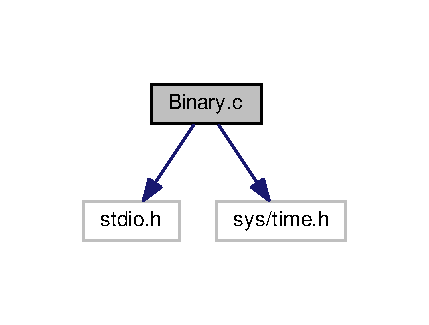
\includegraphics[width=206pt]{Binary_8c__incl}
\end{center}
\end{figure}
\subsection*{Functions}
\begin{DoxyCompactItemize}
\item 
int \hyperlink{Binary_8c_ad2bafc46e8cb458c34c5d4a26a83c68b}{binary1} (int n, int a\mbox{[}n\mbox{]}, int who)
\item 
int \hyperlink{Binary_8c_a2c457548097d2291c438fdb839635616}{binary2} (int n, int a\mbox{[}n\mbox{]}, int who)
\item 
long \hyperlink{Binary_8c_a03534a034bb37b8616529a034a92b389}{timediff} (struct timeval before, struct timeval after)
\item 
int \hyperlink{Binary_8c_ae66f6b31b5ad750f1fe042a706a4e3d4}{main} ()
\end{DoxyCompactItemize}


\subsection{Function Documentation}
\index{Binary.\+c@{Binary.\+c}!binary1@{binary1}}
\index{binary1@{binary1}!Binary.\+c@{Binary.\+c}}
\subsubsection[{\texorpdfstring{binary1(int n, int a[n], int who)}{binary1(int n, int a[n], int who)}}]{\setlength{\rightskip}{0pt plus 5cm}int binary1 (
\begin{DoxyParamCaption}
\item[{int}]{n, }
\item[{int}]{a\mbox{[}n\mbox{]}, }
\item[{int}]{who}
\end{DoxyParamCaption}
)}\hypertarget{Binary_8c_ad2bafc46e8cb458c34c5d4a26a83c68b}{}\label{Binary_8c_ad2bafc46e8cb458c34c5d4a26a83c68b}

\begin{DoxyCode}
11                                       \{
12     \textcolor{keywordtype}{int} left = 0; 
13     \textcolor{keywordtype}{int} right = n-1;
14     \textcolor{keywordflow}{while} (left <= right) \{
15     \textcolor{keywordtype}{int} mid = left + (right-left)/2;
16     \textcolor{keywordflow}{if} (who < a[mid])
17         right = mid - 1;
18     \textcolor{keywordflow}{else} \textcolor{keywordflow}{if} (who > a[mid])
19         left = mid + 1;
20     \textcolor{keywordflow}{else}
21         \textcolor{keywordflow}{return} mid;
22     \}
23     \textcolor{keywordflow}{return} -1;
24 \}
\end{DoxyCode}
\index{Binary.\+c@{Binary.\+c}!binary2@{binary2}}
\index{binary2@{binary2}!Binary.\+c@{Binary.\+c}}
\subsubsection[{\texorpdfstring{binary2(int n, int a[n], int who)}{binary2(int n, int a[n], int who)}}]{\setlength{\rightskip}{0pt plus 5cm}int binary2 (
\begin{DoxyParamCaption}
\item[{int}]{n, }
\item[{int}]{a\mbox{[}n\mbox{]}, }
\item[{int}]{who}
\end{DoxyParamCaption}
)}\hypertarget{Binary_8c_a2c457548097d2291c438fdb839635616}{}\label{Binary_8c_a2c457548097d2291c438fdb839635616}

\begin{DoxyCode}
29                                       \{
30     \textcolor{keywordtype}{int} p = n/2;
31     \textcolor{keywordflow}{while} (n > 0) \{
32     n = n/2;
33     \textcolor{keywordflow}{if} (who < a[p]) \{
34         p -= n;
35     \} \textcolor{keywordflow}{else} \textcolor{keywordflow}{if} (who > a[p]) \{
36         p += n;
37     \} \textcolor{keywordflow}{else}
38         \textcolor{keywordflow}{return} p;
39     \}
40     \textcolor{keywordflow}{return} -1;
41 \}
\end{DoxyCode}
\index{Binary.\+c@{Binary.\+c}!main@{main}}
\index{main@{main}!Binary.\+c@{Binary.\+c}}
\subsubsection[{\texorpdfstring{main()}{main()}}]{\setlength{\rightskip}{0pt plus 5cm}int main (
\begin{DoxyParamCaption}
{}
\end{DoxyParamCaption}
)}\hypertarget{Binary_8c_ae66f6b31b5ad750f1fe042a706a4e3d4}{}\label{Binary_8c_ae66f6b31b5ad750f1fe042a706a4e3d4}

\begin{DoxyCode}
50            \{
51     \textcolor{keywordtype}{int} a[] = \{1,3,5,7,9,11,13,15,17,19,21,23,25,27,29,31,33\};
52     \textcolor{keywordtype}{int} n = \textcolor{keyword}{sizeof}(a)/\textcolor{keyword}{sizeof}(\textcolor{keywordtype}{int});
53     \textcolor{keywordtype}{int} where;
54     \textcolor{keyword}{struct }timeval before;
55     \textcolor{keyword}{struct }timeval after;
56     \textcolor{keywordtype}{int} k;
57     \textcolor{keywordtype}{int} j;
58     gettimeofday(&before, NULL);
59     \textcolor{keywordflow}{for} (j = 0; j < 1000000; j++)
60     \textcolor{keywordflow}{for} (k = 0; k < 2*n+1; k++) \{
61     where = \hyperlink{Binary_8c_ad2bafc46e8cb458c34c5d4a26a83c68b}{binary1}(n, a, k);
62 \textcolor{comment}{//  printf("who = %d, \(\backslash\)tvalue = %d\(\backslash\)n", k, where); }
63     \}
64     gettimeofday(&after, NULL);
65     printf(\textcolor{stringliteral}{"before=[%ld,%ld], after=[%ld,%ld]\(\backslash\)n"}, before.tv\_sec, before.tv\_usec,
66             after.tv\_sec, after.tv\_usec);
67     printf(\textcolor{stringliteral}{"The difference is %ld\(\backslash\)n"}, \hyperlink{Binary_8c_a03534a034bb37b8616529a034a92b389}{timediff}(before, after));
68     printf(\textcolor{stringliteral}{"---------------------------------------------\(\backslash\)n"});
69     gettimeofday(&before, NULL);
70     \textcolor{keywordflow}{for} (j = 0; j < 1000000; j++)
71     \textcolor{keywordflow}{for} (k = 0; k < 2*n+1; k++) \{
72     where = \hyperlink{Binary_8c_a2c457548097d2291c438fdb839635616}{binary2}(n, a, k);
73 \textcolor{comment}{//  printf("who = %d, \(\backslash\)tvalue = %d\(\backslash\)n", k, where); }
74     \}
75     gettimeofday(&after, NULL);
76     printf(\textcolor{stringliteral}{"before=[%ld,%ld], after=[%ld,%ld]\(\backslash\)n"}, before.tv\_sec, before.tv\_usec,
77             after.tv\_sec, after.tv\_usec);
78     printf(\textcolor{stringliteral}{"The difference is %ld\(\backslash\)n"}, \hyperlink{Binary_8c_a03534a034bb37b8616529a034a92b389}{timediff}(before, after));
79     \textcolor{keywordflow}{return} 0;
80 \}\end{DoxyCode}


Here is the call graph for this function\+:
\nopagebreak
\begin{figure}[H]
\begin{center}
\leavevmode
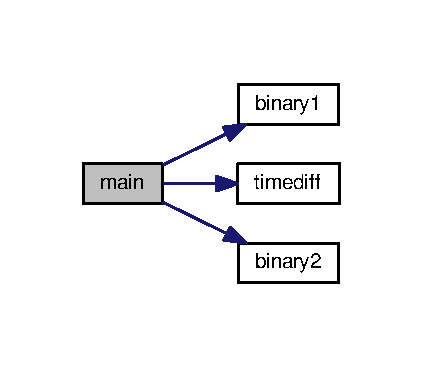
\includegraphics[width=203pt]{Binary_8c_ae66f6b31b5ad750f1fe042a706a4e3d4_cgraph}
\end{center}
\end{figure}


\index{Binary.\+c@{Binary.\+c}!timediff@{timediff}}
\index{timediff@{timediff}!Binary.\+c@{Binary.\+c}}
\subsubsection[{\texorpdfstring{timediff(struct timeval before, struct timeval after)}{timediff(struct timeval before, struct timeval after)}}]{\setlength{\rightskip}{0pt plus 5cm}long timediff (
\begin{DoxyParamCaption}
\item[{struct timeval}]{before, }
\item[{struct timeval}]{after}
\end{DoxyParamCaption}
)}\hypertarget{Binary_8c_a03534a034bb37b8616529a034a92b389}{}\label{Binary_8c_a03534a034bb37b8616529a034a92b389}

\begin{DoxyCode}
44                                                            \{
45     \textcolor{keywordtype}{long} sec = after.tv\_sec - before.tv\_sec;
46     \textcolor{keywordtype}{long} microsec = after.tv\_usec - before.tv\_usec;
47     \textcolor{keywordflow}{return} 1000000*sec + microsec;
48 \}
\end{DoxyCode}

%--- End generated contents ---

% Index
\backmatter
\newpage
\phantomsection
\clearemptydoublepage
\addcontentsline{toc}{chapter}{Index}
\printindex

\end{document}
